% Adam Glogovsky
% Metody inzinierskej prace 2024/25

\documentclass{beamer}

\usetheme{Warsaw}

\usecolortheme{orchid}

\setbeamercovered{transparent}

\usepackage[slovak]{babel}
\usepackage[T1]{fontenc}
\usepackage[utf8]{inputenc}
\usepackage{url}

\usepackage{listings}


\def\BibTeX{\textsc{Bib}\kern-.08em\TeX} 

\newcommand{\footcite}[1]{\footnote{\tiny #1}}
\newcommand{\umlet}{.5}
\newcommand{\emp}[1]{\textit{\alert{#1}}}
\newcommand{\kw}[1]{\mbox{\textbf{#1}}}
\newcommand{\id}[1]{\texttt{#1}}
\newcommand{\stl}{\guillemotleft}
\newcommand{\str}{\guillemotright}

\newcommand{\lsti}{\lstinline[basicstyle=\fontsize{10.5}{12.1}\selectfont]}

\newcommand{\ssection}[1]{
	\section{#1}
	\begin{frame}[fragile=singleslide]\frametitle{}
	\Huge #1
	\end{frame}
}

\newcommand{\ssectionn}[1]{
	\section*{#1}
	\begin{frame}[fragile=singleslide]\frametitle{}
	\Huge #1
	\end{frame}
}

\newenvironment{program}{\begin{beamercolorbox}[rounded=true,shadow=true]{block body}\vspace{-4mm}}{\vspace{-2mm}\end{beamercolorbox}}

\setbeamercolor{fvystup}{fg=white,bg=black}
\newenvironment{vystup}{\begin{beamercolorbox}[rounded=true,shadow=true]{fvystup}}{\end{beamercolorbox}}

\newenvironment{poznamka}{\begin{beamercolorbox}[rounded=true,shadow=false]{block body}}{\end{beamercolorbox}}

\setbeamertemplate{footline}[page number]
{
}



\author{Adam Glogovský}
\institute{
	Fakulta informatiky a informačných technológií\\
	Slovenská technická univerzita v Bratislave}

\subtitle{\vspace{3mm} Metódy inžinierskej práce 2024/2025}

\title{Je odporúčací systém Netflix-u problém?
}

\date{\footnotesize 12. november 2024}




\begin{document}

\begin{frame}[fragile=singleslide]
    \titlepage
\end{frame}


\begin{frame}[fragile=singleslide]\frametitle{Obsah}
    \tableofcontents
\end{frame}


\section{Krátka história}

\begin{frame}[fragile=singleslide]\frametitle{Cena Netflixu}
    Keďže Netflix chcel zlepšiť svôj odporúčací algoritmus, vyhlásil súťaž.
    \begin{itemize}
        \item začala sa v 2009
        \item Snaha o zlepšenie RMSE\footcite{RMSE - root mean squared error - odmocnina priemeru rozdielu medzi reálnymi a očakávanými hodnotami} o 10\%

        \item Už o týždeň tým Bellkor's Pragmatic Chaos prišiel na stanovené zlepšenie
    \end{itemize}
\end{frame}

\begin{frame}[fragile=singleslide]\frametitle{Cena Netflixu}

    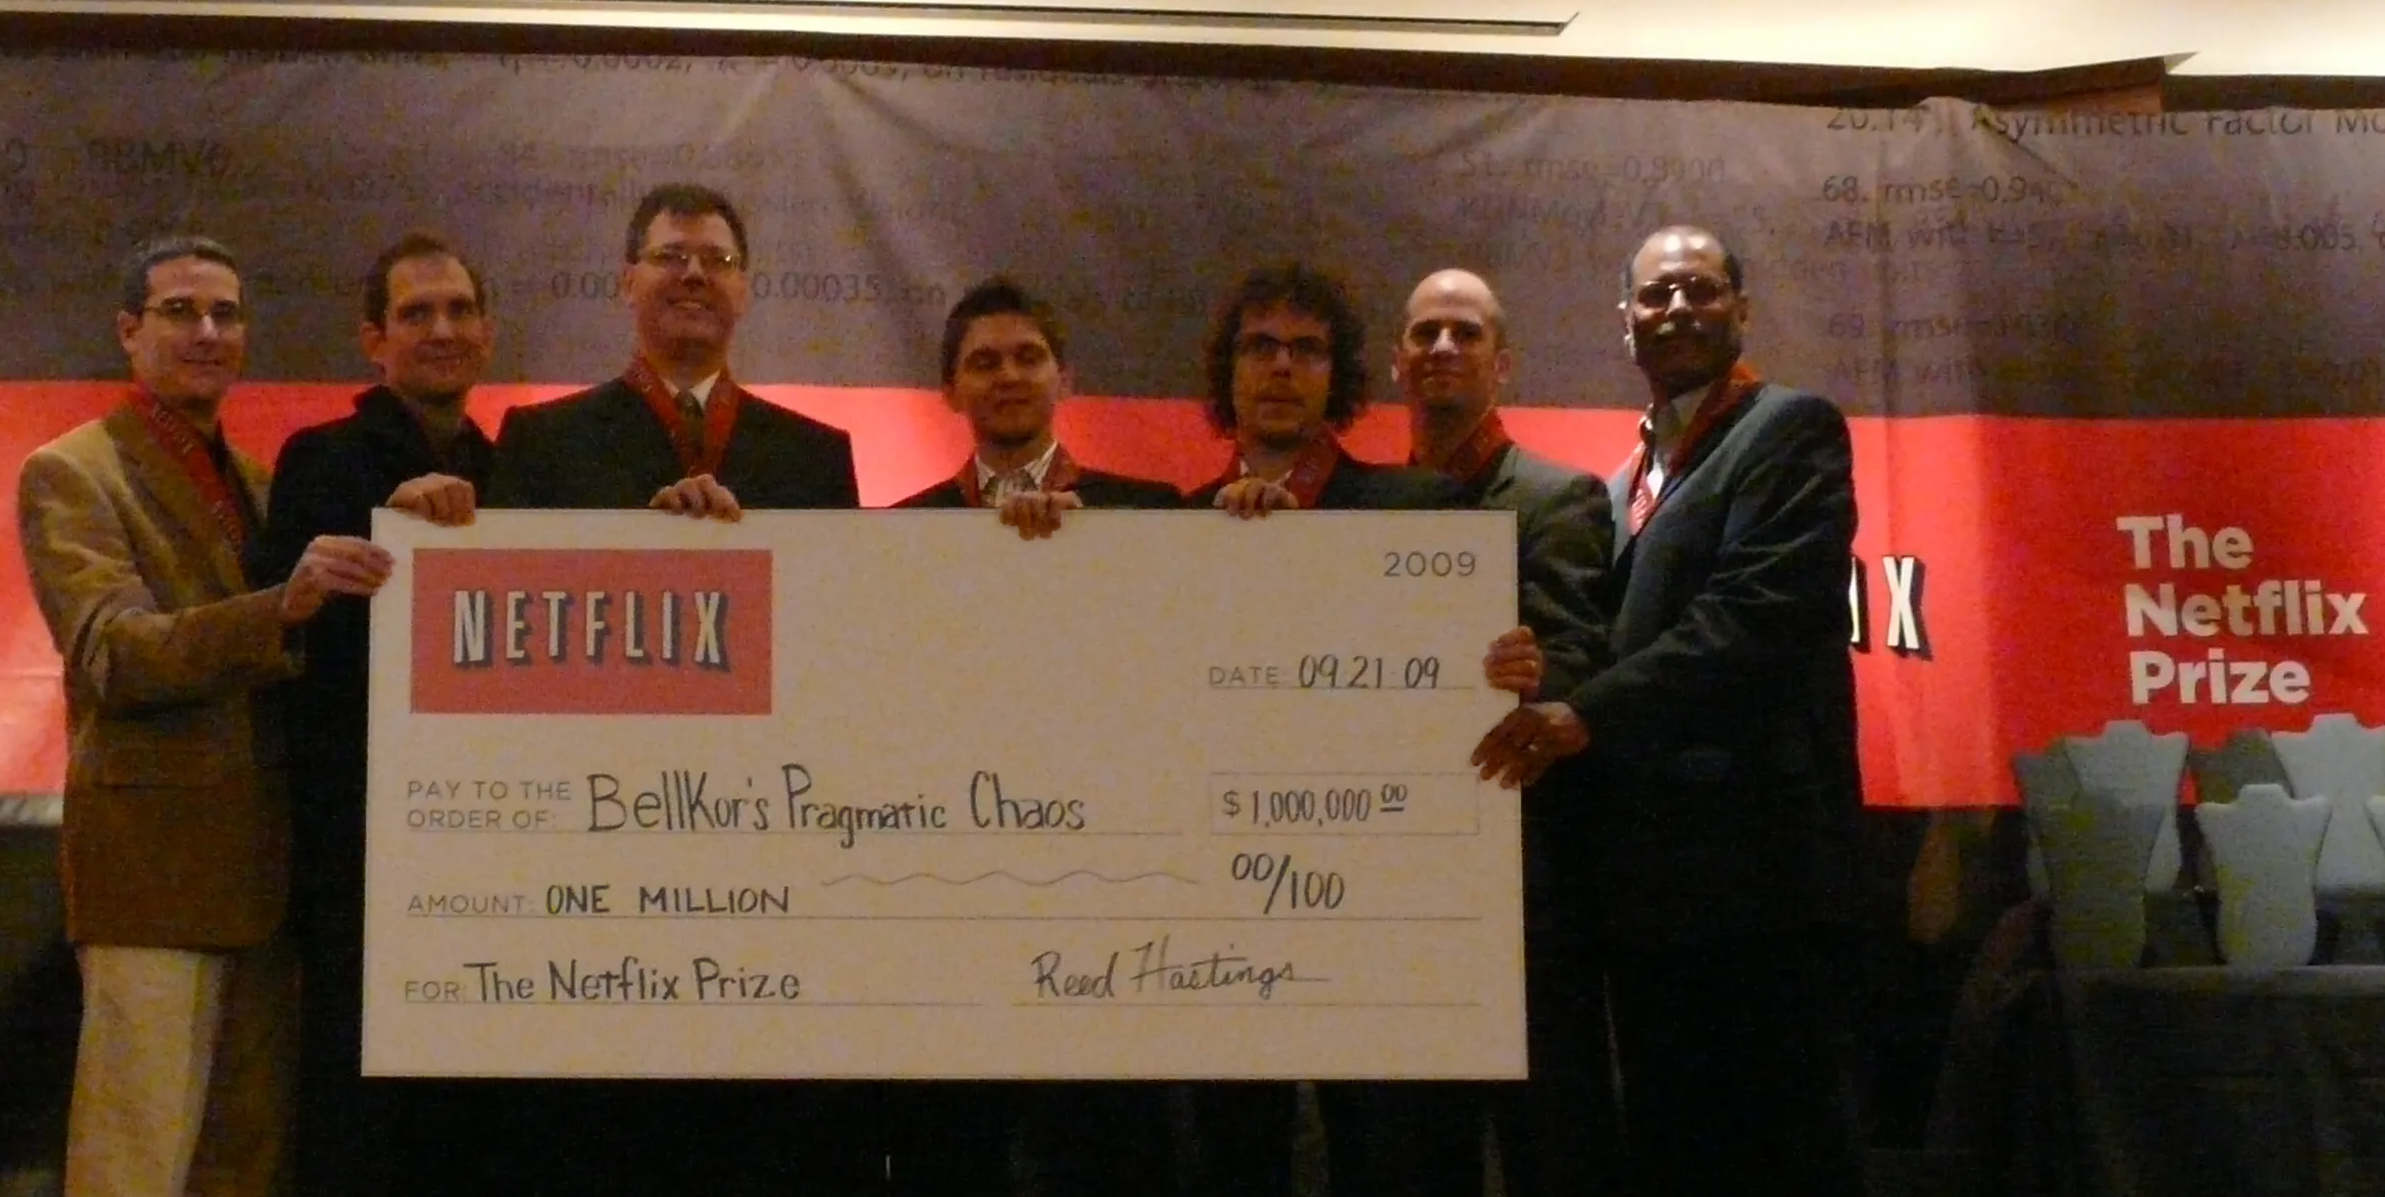
\includegraphics[scale=.13]{NetflixPrize.png}
    {\tiny https://www.wired.com/2009/09/bellkors-pragmatic-chaos-wins-1-million-netflix-prize/}

    {\tiny }
\end{frame}


\section{Problém akváriovej rybky}

\begin{frame}[fragile=singleslide]\frametitle{Problém akváriovej rybky}
    Podľa údajov z Netflixu, ľudia strácajú pozornosť už \textbf{po minúte prezerania si hlavnej stránky.} Týmto sa dozvedeli, že ich úspech stojí a padá na dobrom odporúčacom algoritme.
\end{frame}

\section{Algoritmus}

\begin{frame}[fragile=singleslide]\frametitle{Algoritmus}

    A tak vytvorili celý set alogritmov ktoré riešia veľmi podobné, ale ajtak odlišné problémy.
    \begin{center}
        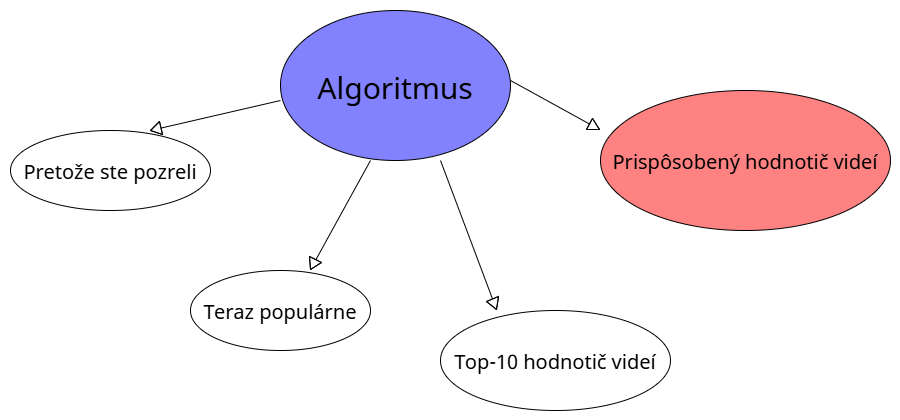
\includegraphics[scale=.3]{DiagramAlgoritmus.png}
    \end{center}


\end{frame}

\begin{frame}[fragile=singleslide]\frametitle{Teraz populárne}
    Je veľmi jednoduchý algoritmus:
    \begin{itemize}
        \item Používaný hlavne na začiatku.
        \item Poukazuje na meniace sa trendy.
        \item Je tam aj troška personalizácie.
    \end{itemize}
\end{frame}

\begin{frame}[fragile=singleslide]\frametitle{Prispôsobený hodnotič videí}
    Najpoužívanejší algoritmus je práve tento. A to pretože:
    \begin{itemize}
        \item Zoradzuje celý katalóg filmov / seriálov pre každý používateľský profil personalizovane.
        \item Jeho cieľ je byť personalizovaný a teda každý by mal dostať to, čo chce.
        \item Jednoducho sa dá upraviť a použiť na iný riadok.
    \end{itemize}
\end{frame}

\begin{frame}[fragile=singleslide]\frametitle{Top-n hodnotič videí}
    Je algoritmus podobný Prispôsobenému hodnotiču videí, s pár rozdielmi:
    \begin{itemize}
        \item Prechádza len najvrchnejšou časťou katalógu filmov/seriálov.
        \item Je personalizovaný, ale viac ho ovplyvňuje lokalita, čas roka a popularita.
    \end{itemize}
\end{frame}




\section{Rozloženie hlavnej stránky}

\begin{frame}[fragile=singleslide]\frametitle{Rozloženie hlavnej stránky}

    
\includegraphics[scale=.26]{NetflixMainPage1.png}

    {\tiny Hlavná stránka}


\end{frame}

\begin{frame}[fragile=singleslide]\frametitle{Jednotlivé riadky}

    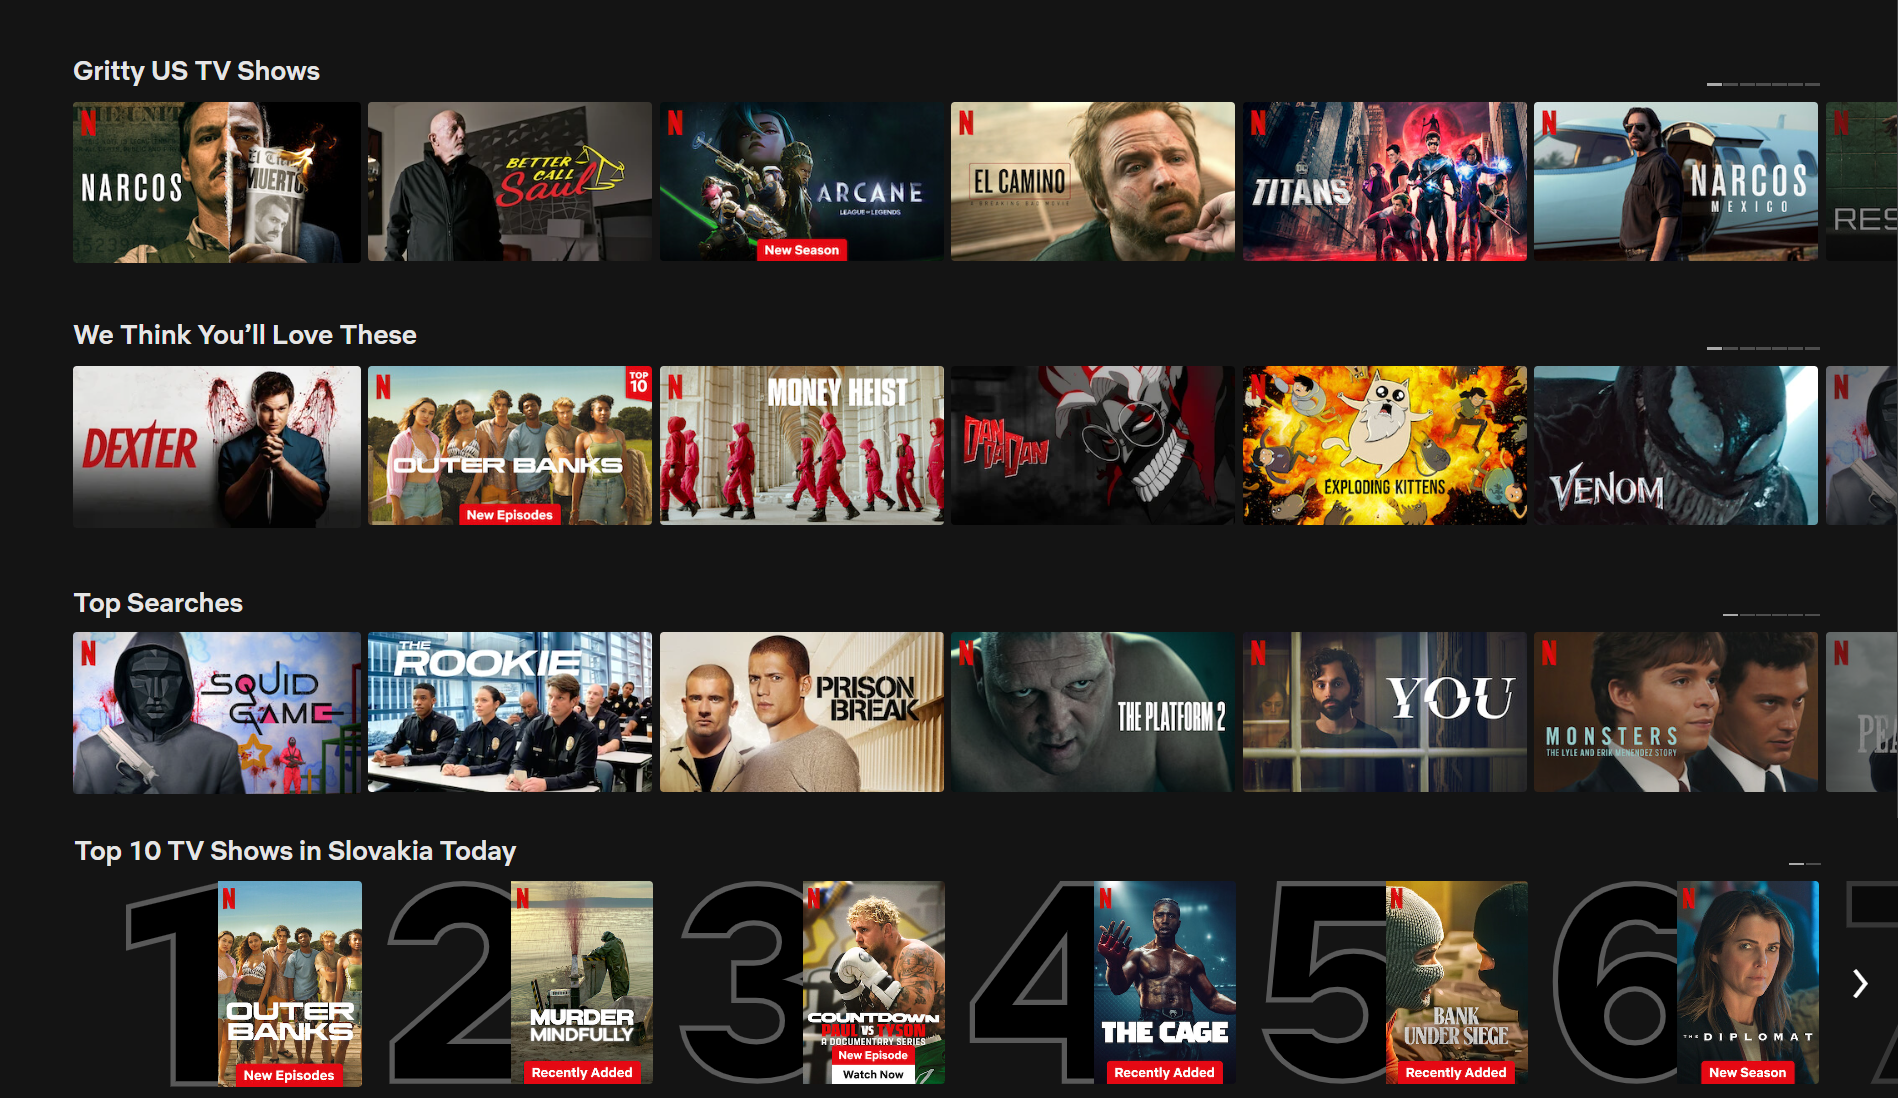
\includegraphics[scale=.26]{NetflixMainPage2.png}

    {\tiny Rozdielne algoritmy pre každý riadok}


\end{frame}

%no a teraz ked uz chapeme ako funguje tento algoritus tak si mozme povedat nieco o jeho dopade
\section{Profitabilnosť}

\begin{frame}[fragile=singleslide]\frametitle{Profit Netflixu}


    \begin{center}
        Peňažná bilancia zisku Netflixu:
        \vspace{0.2cm}

        \begin{tabular}{||c | c||}
            \hline
            Dátum      & Čistý zisk   \\ [0.5ex]
            \hline\hline
            31.12.2020 & 7,57 Mld \$  \\
            \hline
            31.12.2021 & 12,69 Mld \$ \\
            \hline
            31.12.2022 & 17,18 Mld \$ \\
            \hline
            31.12.2023 & 22,59 Mld \$ \\
            \hline
        \end{tabular}
        \footcite{https://ir.netflix.net/financials/annual-reports-and-proxies/default.aspx}

        \vspace{0.4cm}
        Enormný rozdiel hodnoty akcie Netflixu:

        \begin{tabular}{|c | c|}
            \hline
            Dátum      & Hodnota    \\ [0.5ex]
            \hline\hline
            01.11.2023 & 420,19  \$ \\
            \hline
            01.11.2024 & 756,10 \$  \\
            \hline
        \end{tabular}
        \footcite{https://ir.netflix.net/stock-information/stock-chart/default.aspx}
    \end{center}
\end{frame}


\section*{Zhodnotenie}

\begin{frame}[fragile=singleslide]\frametitle{Zhodnotenie}

    \textbf{Takže je teda odporúčací systém Netflix-u problém?.}

    \vspace{1cm}
    Ďakujem za pozornosť!

    \textbf{Priestor pre vaše otázky O:D}
\end{frame}

\end{document}
